\begingroup
\renewcommand{\thefigure}{15.4}
\begin{figure}[htbp]
  \centering
  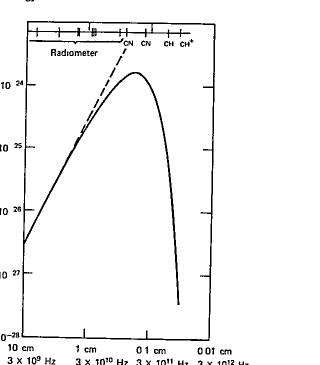
\includegraphics[width=0.58\textwidth]{figures/chapter15/fig15-04.png}
  \caption{Energy density per frequency interval for
  \(2.7^\circ\mathrm{K}\) black-body radiation. The solid curve gives the
  Planck spectrum \eqref{eq:15.5.4}; the dashed line gives the
  Rayleigh--Jeans spectrum \eqref{eq:15.5.7} for an antenna temperature of
  \(2.7^\circ\mathrm{K}\). The short vertical lines mark frequencies at which
  the black-body temperature has been measured or bounded by radiometer or
  interstellar absorption observations.}
  \label{fig:15.4}
\end{figure}
\endgroup
